\documentclass{report}
\usepackage[utf8]{inputenc}

\title{Migrating to Micro Frontends -- Taking it One Step at a Time}
\author{Julius Celik \texttt{<jcelik@kth.se>}}
\date{\today}

\usepackage[euler]{textgreek}

\newcommand{\fe}{\textmugreek FE}

\setlength{\parindent}{0em}
\setlength{\parskip}{1em}

\usepackage{biblatex}
\addbibresource{references.bib}

% For acronyms in the text
\usepackage[printonlyused]{acronym}

% For images
\usepackage{graphicx}

% For blockquotes
\usepackage{csquotes}


\begin{document}

\maketitle

% \begin{acronym}
% \acro{DX}{Developer Experience}
% \acro{UX}{User Experience}
% \end{acronym}
% 
\chapter{Introduction}

\section{Background}
\acp{MFE} is a web \ac{FE} architecture style, where the \ac{FE} is composed of multiple simultaneously running applications. As the name implies it is heavily inspired by the microservice architecture style. It promises \ac{DX} improvements similar to those that microservices provide, like team independence, clear code responsibility, and high cohesion. Additionally \acp{MFE} promises a higher cohesion between \ac{BE} and \ac{FE}, mitigating feature latency that comes from asynchronous deployment. In practice this means that the delay from starting to implement a feature to it reaching market, should be decreased when using \acp{MFE} \cite{Celik}. \textbf{ADD SOURCES!!!}


\section{Problem Statement}

Write about how teams should be very divided and independent

Write about how teams would like to try \ac{MFE} but should not edit code from other teams.

\section{Problem}

Is it possible to implement \ac{MFE} without changing other parts of the code base? Access transparency and self contained micro frontends. Three artifacts are introduced:

\begin{description}
\item[Construct] Self contained micro frontends.
\item[Instantiation] Plutt -- A build tool for self contained micro frontends.
\item[Method] The method of creating self contained micro frontends.
\end{description}


\textbf{Old problem}

The feasibility of \acp{MFE} are unknown, as the performance impacts are not known. It is believed that \ac{DX} could be improved by using \acp{MFE}, but the technology is criticised for possibly introducing a large negative performance impact, which in turn affects \ac{UX}.


It would be interesting to measure the \ac{UX} performance impact when using \acp{MFE}. If it could be shown that a complex production facing web application could be transformed, to use a \ac{MFE} architecture \textit{without} a significant performance impact, the criticism regarding performance can be rejected. The problem can be condensed into the following research question:

\begin{center}
\begin{tabular}{p{0.28\textwidth}p{0.60\textwidth}}
     \textbf{Research Question:} & Is it possible to transform a monolithic complex production facing web application, to use a \ac{MFE} architecture, without \ac{UX} being significantly affected?
\end{tabular}
\end{center}

\section{Hypothesis}
It is possible to implement a monolithic complex web application using a \ac{MFE} architecture, without a large negative impact on performance and \ac{UX}.

\section{Purpose}
The purpose is to evaluate the feasibility of using \acp{MFE}, regarding \ac{UX}. The impact on \ac{DX} will not be evaluated. Assuming that \ac{DX} is positively impacted, there is a value in knowing if there is a trade-off between \ac{DX} and \ac{UX} or if \ac{UX} impacts are negligible.

\section{Goal}
The goal is to try to transform a monolithic complex web app, to using a \ac{MFE} architecture and compare performance between the monolithic web page and the \ac{MFE} web page. The attempt is that the \ac{MFE} page will have similar performance to the monolithic page, as this would mean that only \ac{DX} has to be considered when evaluating the use of \acp{MFE}.

\section{Tasks}
Initially a literature study will be conducted with two purposes:

\begin{enumerate}
    \item Evaluate the different methods for implementing a \ac{MFE} architecture.
    \item Decide on quantifiable performance metrics that have shown an impact on \ac{UX}. Likely metrics could be bundle size, time to first interaction, or time to first render. As there exists extensive research into this field, the chosen metrics will be a very trustworthy measurement of \ac{UX} impact.
\end{enumerate}

When an implementation and evaluation method is chosen, a complex monolithic web application will be re-implemented, using a \ac{MFE} architecture. When the modified web page is created the original and modified page can be compared, using the chosen performance metrics.

Finally the results will be evaluated and analyzed. The research question will be answered. All of this will be compiled into the thesis.

\section{Research Methodology}

\section{Old Method}
The project will use an empirical method. There exists quantifiable measurements, and the correlation between these and \ac{UX} are very extensively proven. Therefore, there exists a good foundation for conducting performance tests on web pages, and then from analysis of these measurements deduce \ac{UX} impact.

The biggest flaw with the chosen method is that it does not provide any method for proving that \acp{MFE} lead to a negative \ac{UX} impact. If the modified page is significantly worse than the original page it only proves that this specific page became worse, which could be because of a poor implementation. If the modified page has similar performance as the original page it proves that it is possible to create a \ac{MFE} web page with no significant performance degradation. Therefore, the hypothesis can be proven, but not rejected.

\section{Supervisor and Examiner}

My supervisor from KTH will be Martin Monperrus. My examiner from KTH will be Benoit Baudry.

The project will be conducted at DigitalRoute who will provide Tommy Gunnarsson as a supervisor. They will also provide me with any necessary equipment like a computer, and access to all of the development tools used at DigitalRoute.

\section{Eligibility and study planning}

All my courses from my bachelor are completed. I have completed more than 60 credits of advanced courses in my master. During my master thesis, I will conduct one 7.5 credit course, and after my master thesis I will have finished all courses for my master.

\section{Milestone chart}

The project will start on 13 January and end on 29 May. There will be the following milestones:

\textbf{7 February:} The project plan and literature study is finished. At this stage the method for implementation and performance evaluation will be chosen.

\textbf{17 April:} The modified web page will be finished. At this stage performance tests can be conducted.

\textbf{15 May:} The first draft of the Thesis will be finished. If it is accepted a thesis presentation date can be chosen.

\textbf{22 May:} The project presentation has been conducted and peer reviews have been provided.

\textbf{29 May:} The final thesis report is submitted.

\chapter{Background}

\textbf{TODO introduce chapter}

\textbf{lorem ipsum}

\textbf{Maybe mention transparencies somewhere}

\section{HTLM and the DOM}

Web pages are composed of \ac{HTML} and \ac{CSS} documents. \ac{HTML} and \ac{CSS} are declarative programming languages that define the content and styling of web pages \cite{Lie1999}. This means that the \ac{GUI} of a web page is defined by the content of the corresponding \ac{HTML} and \ac{CSS} documents. As \ac{HTML} and \ac{CSS} can be seen as being complementary technologies, and is often used together, all uses of \ac{HTML} will be a reference to both \ac{HTML} and \ac{CSS} for the rest of the thesis. \ac{HTML} was both meant to be written by humans, and generated by computer applications (front-end applications) \cite{Lie1999}. The process of when a front-end application generates \ac{HTML} documents is called rendering.

Front-end applications can be categorized into 5 categories, which are presented in Figure \ref{fig:fe-render-methods}. They are categorized on when, and how close to the client device, the rendering process is executed. Static \ac{HTML} is when a developer manually writes \ac{HTML}. Pre-rendering is when a developer uses another markup language than \ac{HTML}, and then uses a tool to render the markup into \ac{HTML}. The server in this case, where the render is performed, does not necessarily have to be the same server that serves the \ac{HTML} to clients. It is used to describe a computer that is not the client. Pre-rendering is done either for a simpler development process, or for use cases that require a larger feature set than static \ac{HTML} can provide. Server Side and Client Side Rendering is when \ac{HTML} is rendered in run time, which is often done for dynamic content or interactive behaviour. Different rendering methods can be mixed for different parts of a web page. If both server side and client side rendering is used for the same parts, it is called Isomorphic rendering.

\begin{figure}
    \centering
    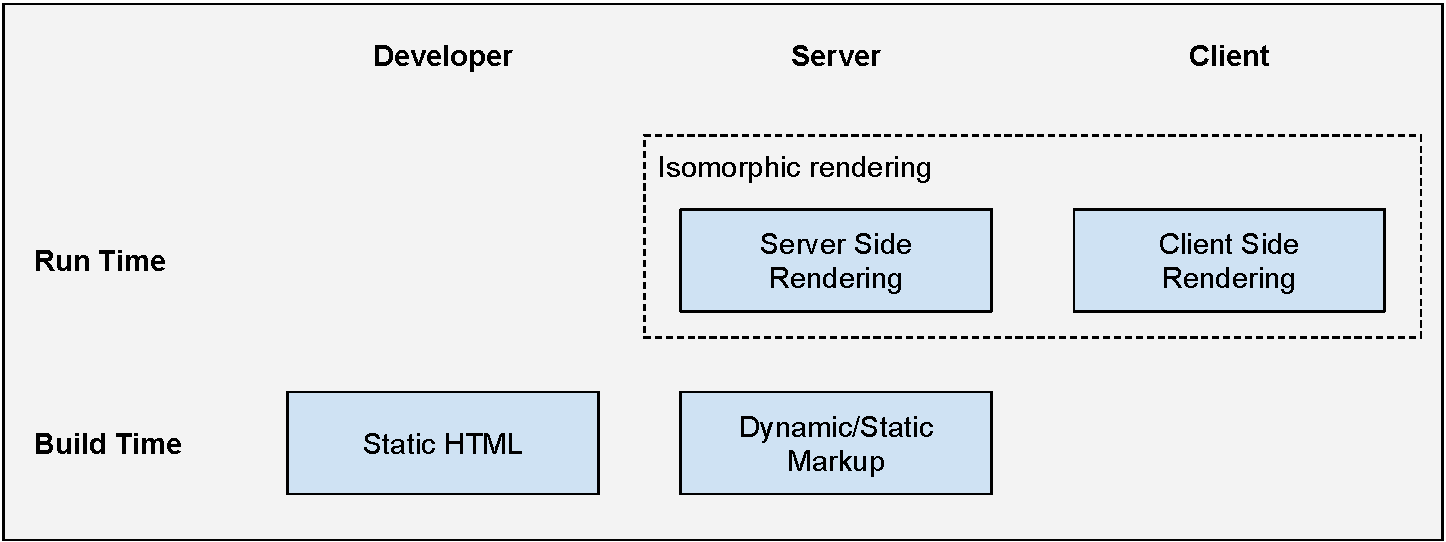
\includegraphics[width=\linewidth]{images/fe-rendering.pdf}
    \caption{Different methods for generating \ac{HTML}. When it is done by a server or client device it is called rendering. Multiple methods can be used for the same web page, and if it is done using different methods, for the same part of the page, it is called isomorphic rendering.}
    \label{fig:fe-render-methods}
\end{figure}

\subsection{Pre-rendering and Server Side Rendering}

Pre-rendering static markup is when tools are used that transform files from one markup format into \ac{HTML}. This is often done in build-time. Pandoc is a tool that translates simpler markdown formats to \ac{HTML} \cite{Dominici2014}. The most prominent benefit is that more lightweight markup languages can be quicker and easier to use when developing web pages as they are more human readable and less verbose, at the cost providing a more limited feature set \cite{Dominici2014}.

There also exists markup languages like PHP that provide a larger feature set than \ac{HTML}. These can provide imperative programming constructs that allow access to perform network calls, composition of reusable components, or resolve database queries \cite{Royappa2000}. These front-end applications can execute their render both in build-time or run-time, depending on if they have to provide dynamic content based on the client request. Dynamic refers to the dynamic nature of the content, where the content is mutable, persistent or user customized. If the render is executed in build time it is pre-rendering based on dynamic content, and if it is done in run time it is called server side rendering.

\subsection{Client Side Rendering}

A front-end application can also be client based where a client receives one or many scripts, that manipulate the \ac{HTML} document. This results in \textit{interactive} applications where user interactions result in animations or GUI changes, without a page refresh. To facilitate this, browsers expose an API, called \ac{DOM}, that allows scripting languages to access and manipulate \ac{HTML} documents \cite{Apparao1998}. This is most commonly done using JavaScript. Already in the beginning of the 2000's researchers experimented with client side rendering, where JavaScript was used to update the \ac{GUI} without a page refresh \cite{Betz2000}.

\textbf{AJAX and asynchronous updates.}

Client side rendering can also be used to render all of the content of a web page, and even simulate page navigation by re-rendering most or all of the web page. This type of front-end application is called \ac{SPA}, because of how the full front-end application is included in one page \cite{Mesbah2007}. Sometimes the different navigation methods are called hard and soft navigation, where soft navigation is when the navigation is simulated by a client side front-end application.

All different front-end applications methods can be mixed where different parts of the \ac{HTML} document is rendered using different methods. If the same parts are rendered both by the server and the client, it is called \textit{isomorphic rendering} \cite{Brehm2013} or universal application \cite{alabes2017isomorphic}. The concept is that a web page is first rendered at the server, sent in a rendered state to the client, and then a replica of the front-end application is sent to the client. When the replica has been loaded on the client, the web page is re-rendered and acts as a traditional \ac{SPA}. The benefit compared to a traditional \ac{SPA} is that the web page is loaded quicker, as the initial file contains all required \ac{HTML} to show the web page \cite{Brehm2013}. It also improves search engine performance, and allows users to optionally use JavaScript\cite{Brehm2013}.

\section{Modern web development}
\subsection{Patterns}
\textbf{discuss modern web applications. Props down, events up. One way data flow}
\subsection{Tools}
\textbf{react/vue, webpack/babel, node, npm/package.json, typescript}

\section{Component Composition}

\textbf{Write about all kinds of approaches to compose a gui of multiple components. Preferably in run time.}

\textbf{Portlets and Mashlets (web mashups)}

\textbf{Transclusion}

\section{Microservices (this section will be re-written)}

\textbf{Focus more on what microsercvices are. The definition.}

Microservices is a software development method where systems are divided into smaller parts, called microservices, that can be individually deployed \cite{Newman2015a}. In turn, this enables low coupling, high cohesion, and strong composability \cite[ch.~1]{Newman2015a}. It also enables multiple developers to work on a shared codebase while minimizing obstruction, which becomes more notable in larger systems, with a large number of developers \cite{Newman2015a}. This concept is also referred to as team independence.

% Microservices are focused on performing single tasks really well, and implementing functionality by composing multiple microservices.

A central aspect of microservices is the concept of ``vertical slicing'' as a decomposition strategy, which is an important facilitator of team independence \cite{Familiar2015}. An example of vertical slicing can be seen in Figure \ref{fig:vertical-slicing}. An early adopter of vertical slicing was \citeauthor{Ratner2011} who observed agile teams who broke up user stories into multiple horizontal layers. They observed that teams focused on one part of the technology stack at a time, which resulted in stories that provided non user facing changes. Vertical slicing solves this by defining stories and responsibilities that encompass end-to-end functionality. This means that instead of thinking in terms of user interface, business logic, and data storage as separate distinct horizontal layers, a story should include all of them, but only from a narrow context \cite{Ratner2011}. \citeauthor{Ratner2011} describes their method as \blockquote{[...] driving a thin vertical slice from UI to database, which is functionally coherent and demonstrable, then progressively widening it with consecutive slices. \cite{Ratner2011}}

\begin{figure}
    \centering
    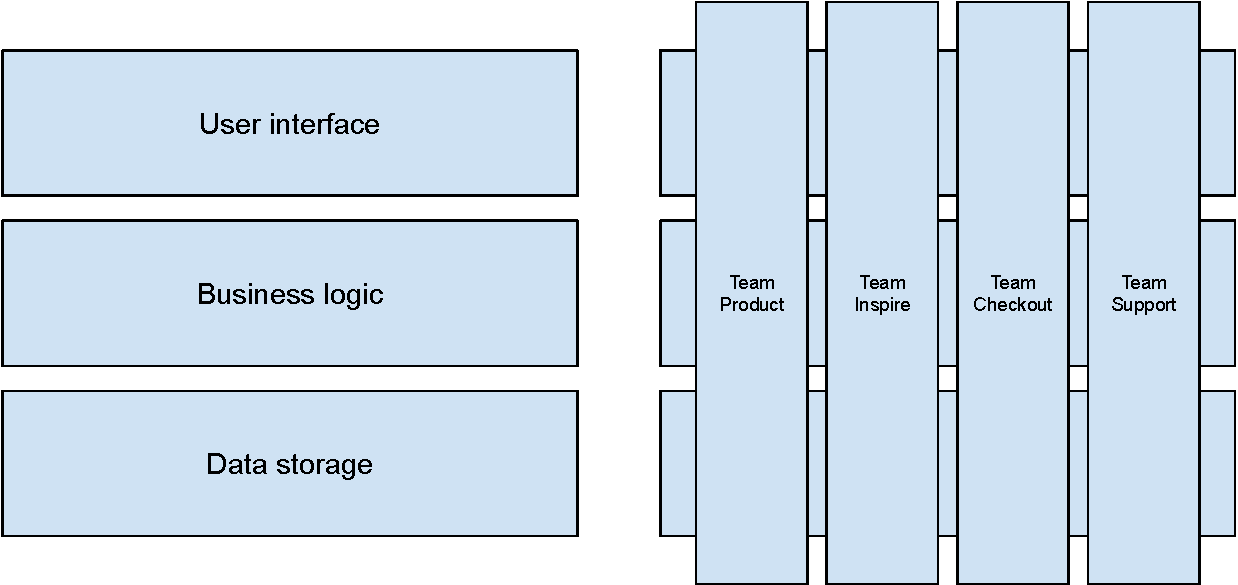
\includegraphics[width=\linewidth]{images/vertical-slicing.pdf}
    \caption{Horizontal Layering and Vertical Slicing. This is an example of four cross functional development teams that are responsible for all aspects of delivering a customer facing feature.}
    \label{fig:vertical-slicing}
\end{figure}

Vertical slicing can be applied to stories like \citeauthor{Ratner2011} describe \cite{Ratner2011}, to team responsibilities, and to system design \cite{Geers2020}. Vertical slicing is a consequence of cross functional agile teams \cite{Geers2020}, which can be explained by Conway's law: \blockquote{Any organization that designs a system (defined broadly) will produce a design whose structure is a copy of the organization's communication structure \cite{Conway}.} This can be interpreted as vertical slicing of system components being a consequence of smaller cross functional teams.

\section{Semantic Versioning and Lock-step Deployments}

See page 64-65 in ``Building Microservices (Sam Newman)''

Gradual Migration

\section{Vertical Decomposition and Self-Contained Systems}
\chapter{Related work}


\section{Micro Front-ends}

Micro front-ends is a front end technique that originates from microservices \cite{Jackson2019}. Where microservices aim to solve scalability problems in the back-end, micro front-ends aim to solve the same problems in the front-end, by applying many of the same concepts and methods. There does not exist one single definition, but one of the introducers of micro front-ends, ThoughtWorks, defines micro front-ends as: \blockquote{An architectural style where independently deliverable front-end applications are composed into a greater whole \cite{Jackson2019}}

An essential common aspect, between microservices and micro front-ends, is the possibility for independent deployability \cite{Jackson2019}, where teams can deploy any changes to software owned by them, without having to coordinate with other teams. The way this is achieved is by using vertical slicing, a software decomposition strategy, based on composing software in functionally coherent slices that fully implement features \cite[ch.~1]{Geers2020}. Using vertical slicing aims to limit the boundary surface areas between different teams' code. Some of the promised benefits of using micro front-ends are simple decoupled codebases, independent deployment, autonomous teams \cite{Jackson2019}, and better customer focus \cite[ch.~1]{Geers2020}.

\citeauthor{Geers2020} presents the evolution of decomposition strategies as in Figure \ref{fig:evolution-of-decomposition-strategies}. Monoliths means that an application is fully included in one code base, and process. An intuitive decomposition is to decompose the front-end from the back-end, which leads to front-end developers being able to work more independently from the back-end. When teams grow it has become more common to divide the monolithic back-end into a vertically sliced microservice back-end. \citeauthor{Geers2020} proposes that it is a natural progression to continue the progress into vertical slices that spans both the back-end and the front-end, which are micro front-ends \cite{Geers2020}.

\begin{figure}
    \centering
    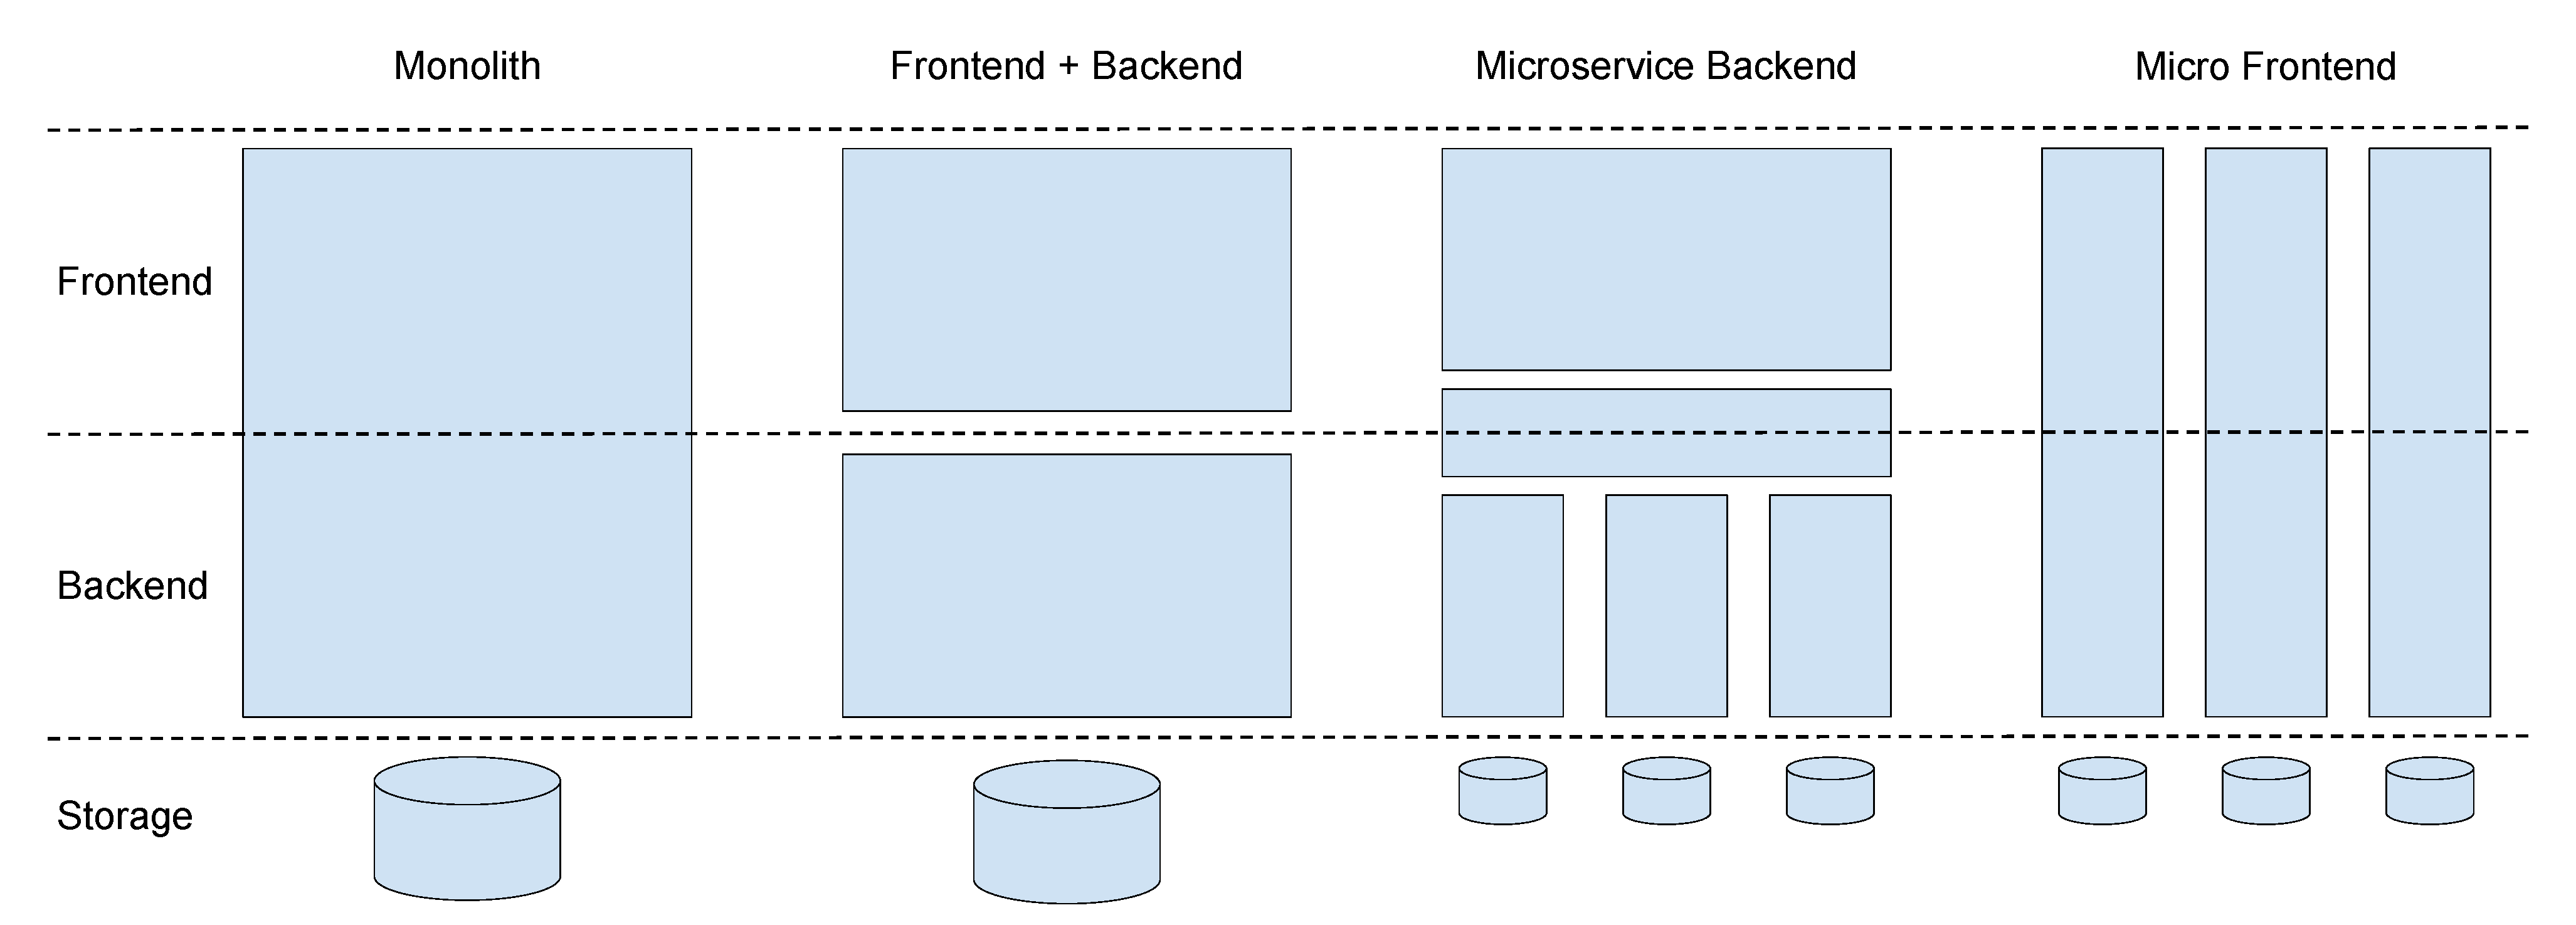
\includegraphics[width=\linewidth]{images/evolution-of-decomposition-strategies.pdf}
    \caption{An Evolution of Decomposition Strategies}
    \label{fig:evolution-of-decomposition-strategies}
\end{figure}

Even though \citeauthor{Geers2020} preferably envisions micro front-ends as fully vertically aligned with the back-end, that does not have to be the case. Many micro front-ends exist apply the architecture patterns of microservices, without being fully aligned with the back-end. Figure \ref{fig:micro-frontend-alignment} presents three approaches to aligning a micro front-end to a back-end. A \textit{Shallow Micro Front-end} is a micro front-end that is in no way aligned to the back-end. The back-end can be one monolith, microservices behind one API-Gateway or multiple services. Based on Conway's law, this probably also means that there exists development teams that work only on the back-end or only on the front-end \cites{Conway}. A \textit{Vertically Aligned Micro Front-end} is when there is a dedicated back-end service that the micro front-end primarily communicates with. A \textit{Monolithic Micro Front-end} is when a micro front-end is a part of a server side rendered monolith, where the back-end and front-end is delivered in one monolithic application. These

\begin{figure}
    \centering
    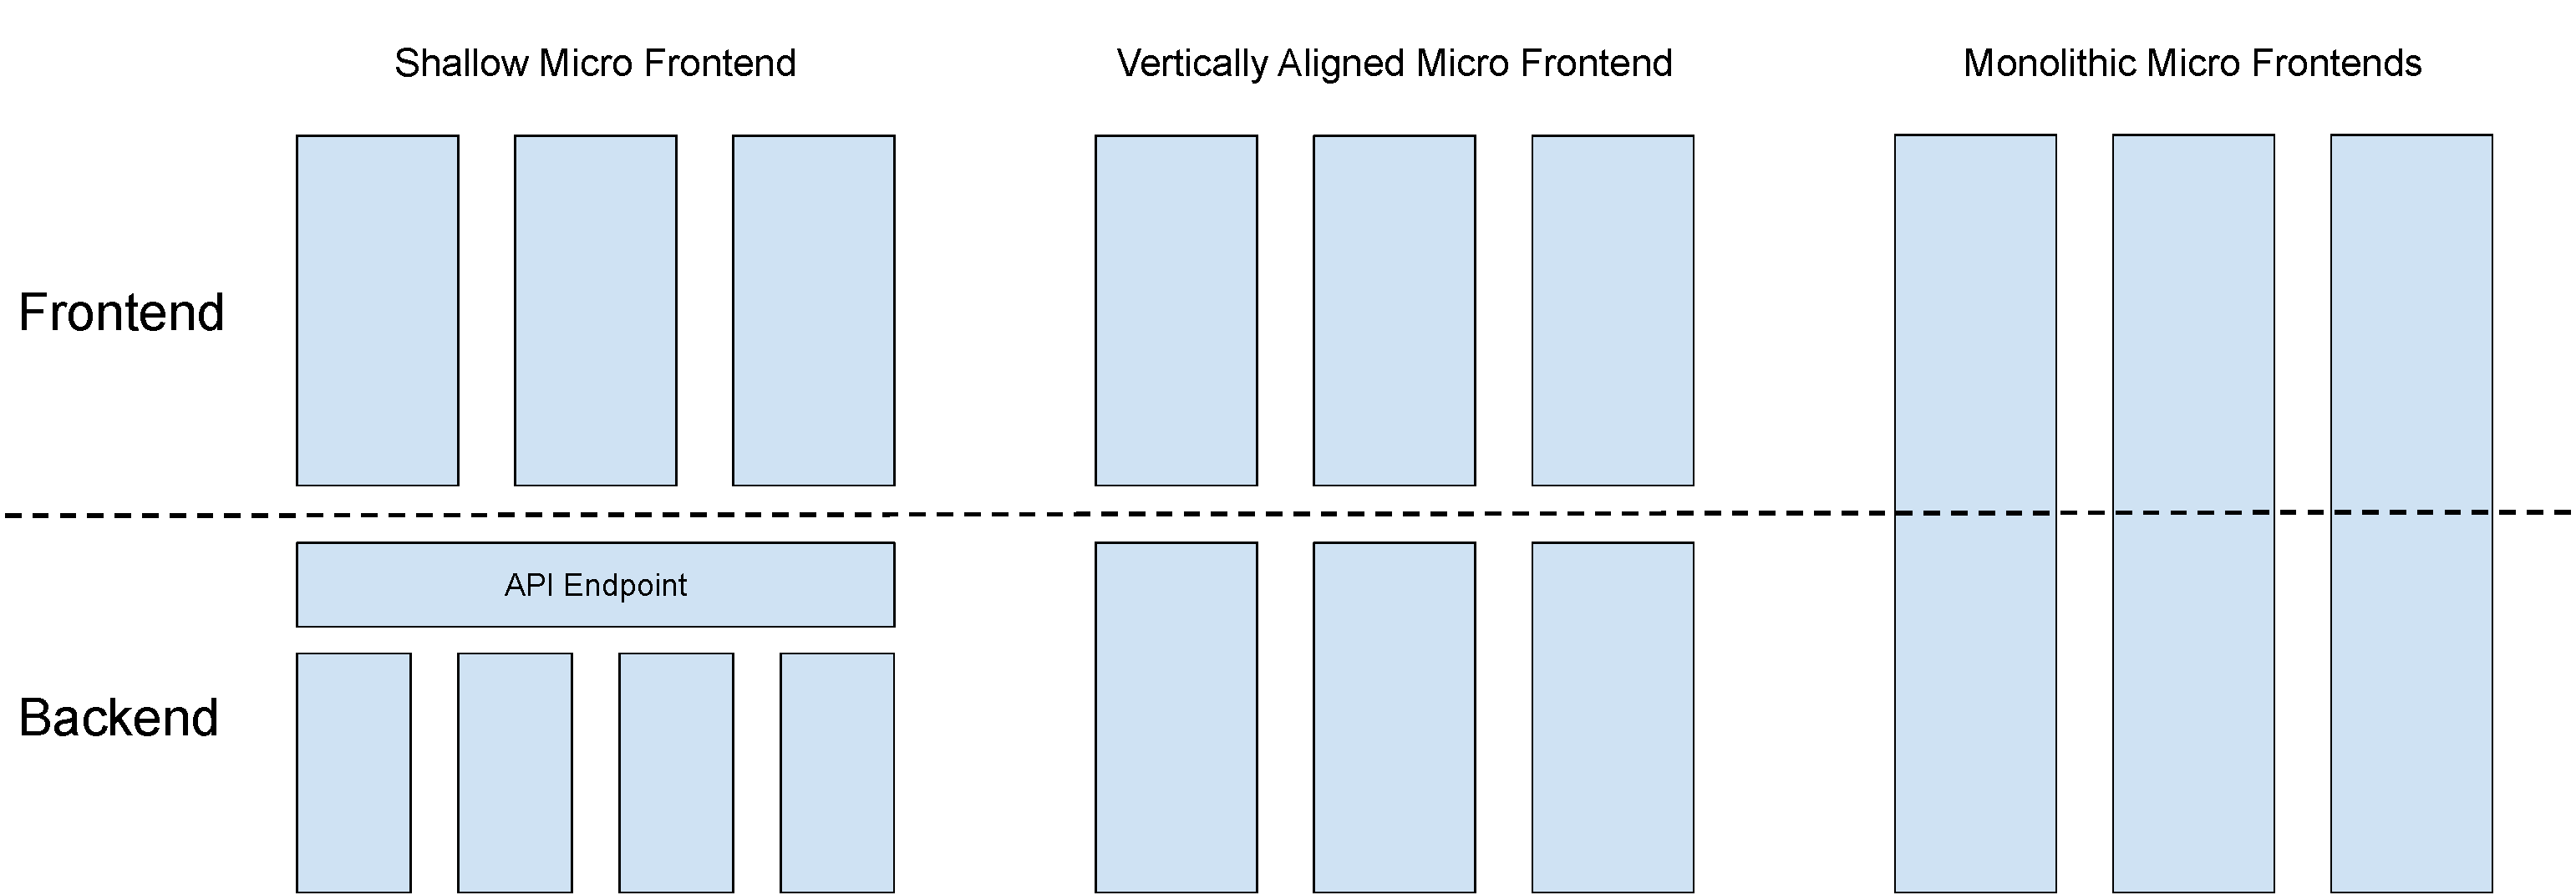
\includegraphics[width=\linewidth]{images/micro-frontend-strategies.pdf}
    \caption{Micro Front-end strategies}
    \label{fig:micro-frontend-alignment}
\end{figure}


\section{Pages and Fragments}

There are many different methods for composing micro front-ends into one coherent front-end. A very important distinction is also to differentiate between micro front-ends that are \textit{pages} or \textit{fragments}. All front-ends are composed by one or more pages. In this case a page refers to a full application view, that covers the full application window. A user can not view multiple pages simultaneously. A fragment is an element of a page. A fragment can be a button, a navigation bar or any other graphical components. A page can include many fragments.

Figure \ref{fig:fragment-page} exemplifies the concept. In this example, the front-end is composed of two pages, which can be served on two different routes. The pages are composed of fragments, and some of the fragments are identical on both pages.

\begin{figure}
    \centering
    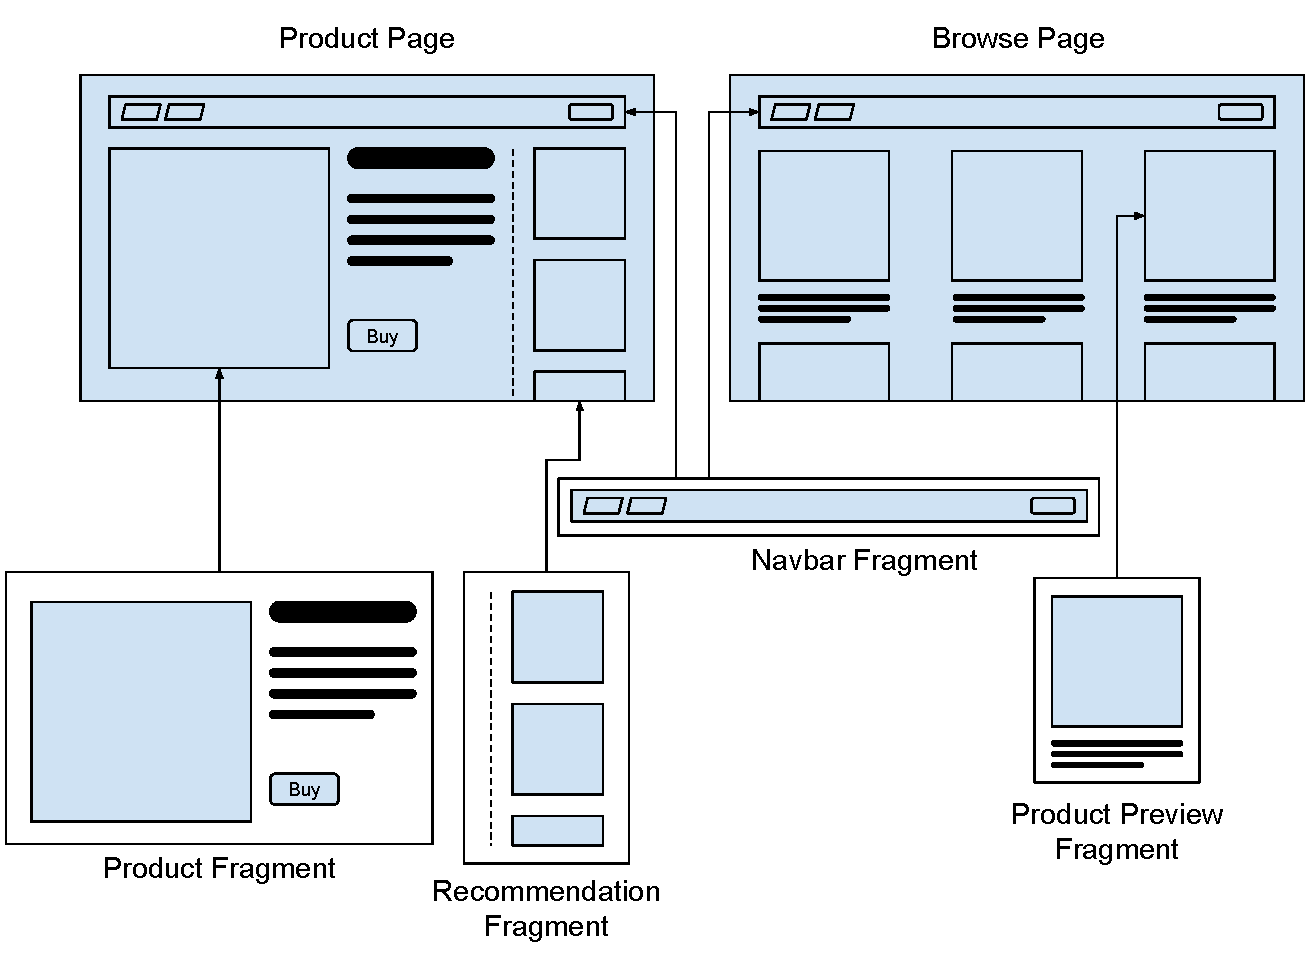
\includegraphics[width=0.9\linewidth]{images/fragment-page.pdf}
    \caption{An example of an e-commerce web page. It consists of two pages, and four fragments, where one fragment is reused on both pages.}
    \label{fig:fragment-page}
\end{figure}

The definition of a fragment is purposefully left vague as ``a part of a page''. The granularity is not specified, which means that multiple fragments in the example could be defined as one fragment, or that a fragment can be divided into multiple fragments. This also implies that a page is an edge case of one large complex fragment.

\section{Composing Micro Front-ends}

As a user uses an application the front-end has to be a coherent application, which means that different micro front-ends has to be integrated into a cohesive experience. Some differentiating questions that arise are ``when and where are the micro front-ends composed?'' The following sections aim to answer those questions. Note that micro front-end \textit{composition} is different from \textit{rendering}, which is when code is evaluated into HTML and CSS code. Composition is the process of integration multiple micro front-ends into one cohesive front-end.

\textbf{mention portlets}

\subsection{When are micro front-ends composed?}

Using ThoughtWorks definition of micro front-ends a micro front-end can be composed both in build-time and run-time \cites{Jackson2019}. Other definitions define micro front-ends as being composed in run-time \cite{Geers2020}. There exists a consensus that using build-time integration loses many of the benefits of using micro front-ends, like independent deployability \cite{Jackson2019}. It is also such a broad definition that most web pages could be defined as micro front-ends. For those reasons, only run-time composition will be considered.

\subsection{Where are micro front-ends composed?}

Micro front-ends can be integrated on the server, on the client, or a combination of both \cite{Jackson2019}. The simplest server side integration is to serve different web pages on different routes \cite{Jackson2019}. All traditional tools and processes can be used to develop the separate pages, and the different micro front-ends can be \acp{SPA}. This can be achieved with a web proxy to serve the different pages on a single domain address, which is visualized in Figure \ref{fig:web-proxy-example}.

\begin{figure}
    \centering
    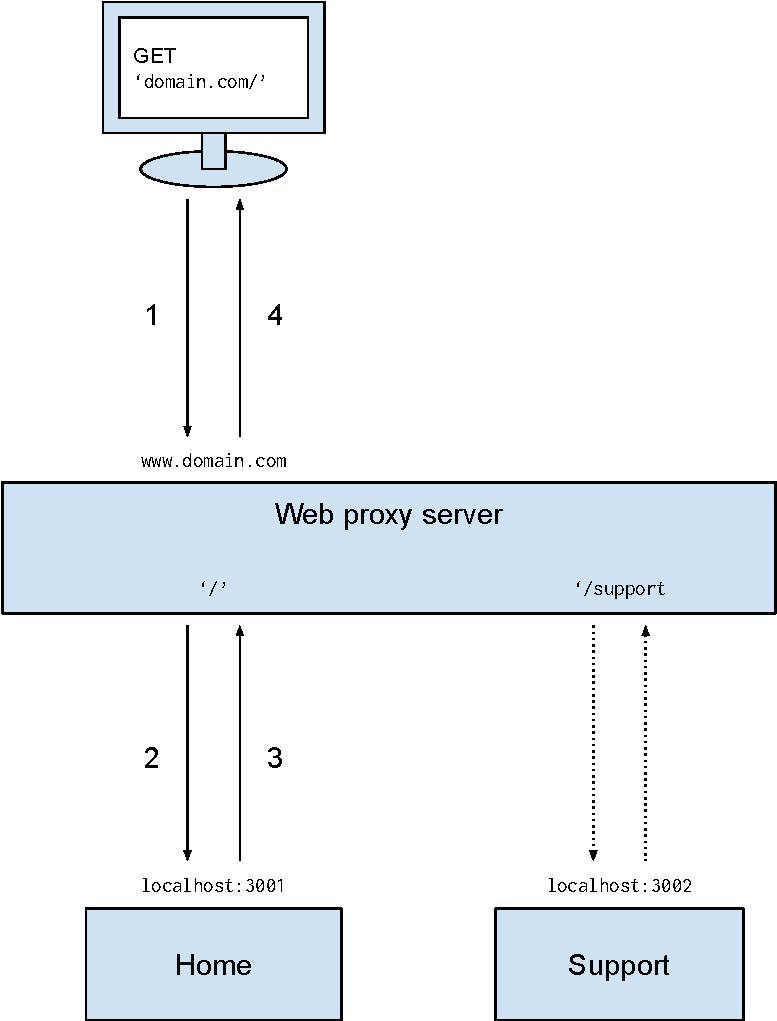
\includegraphics[width=0.5\linewidth]{images/web-proxy.pdf}
    \caption{A web proxy that redirects HTTP requests depending on the route requested. The web servers do can be developed with any existing mature web technology, without having to consider the other servers.}
    \label{fig:web-proxy-example}
\end{figure}

Server side integration can also be used to serve page fragments. This is sometimes called transclusion, and can be done by using technologies like Server Side Includes, Edge Side Includes, Zalando Tailor, or Podium \cite[ch.~4]{Geers2020}. Note that as pages just are large fragments, these technologies can also be used to divide an application on a page level.

All existing client side integration methods can be used for fragment composition, and therefore page composition. The most naive client side integration method is using iframes, which is a web-native standard \cite[ch.~2]{Geers2020}. Iframes were introduced with the HTML 4.01 standard in 1998 \cite{Raggett1999}, when web was still an early technology, which is why there are drawbacks to using them on a modern web app. The most notable trade-offs are performance overhead, accessibility problems, search engine optimization problems, and the lack of layout control \cite[ch.~2]{Geers2020}.

A much newer web-native standard is web components, which in practice is a suite of four web technology standards \cite{MDNWebDocs}. They allow dynamic custom elements to be defined and registered, in an encapsulated scope \cite{MDNWebDocs}. They are used by Google on large products like Youtube to include highly interactive elements \cite{ThePolymerProjectc}.

Figure \ref{fig:web-components} shows an example of how an example web component is created, defined, and what the \ac{DOM} is evaluated into. There are fewer drawbacks with using web components compared with using iframes, but some still exist. The largest issue is that web components do not server side rendering, as they have to be run in a browser at the client \cite[ch.~5]{Geers2020}. This issue can become a problem for performance, accessibility, and search engine optimization. Another drawback, compared with using build-time integration, is the lack of static annotations and analysis. Web components can be internally statically analyzed, but there does not exist any mechanism to share static annotations across the boundary of a web component.

\begin{figure}
\centering
\begin{subfigure}{.65\linewidth}
  \centering
\begin{lstlisting}[
basicstyle=\fontsize{7}{9}\selectfont\ttfamily,
breaklines=true,
frame=single
]
<html>
  <body>
    <my-component></my-component>

    <script>
class MyComponent extends HTMLElement {
  connectedCallback() {
    this.innerHTML = `<h1>Hello!</h1>`;
  }
}

customElements.define(
  'my-component',
  MyComponent
);
    </script>
  </body>
<html>
\end{lstlisting}
  \caption{An example of how to use custom elements. First the class \texttt{MyComponent} is defined, and registered on the name \texttt{my-component}. Then all instances of \texttt{my-component} is replaced on the \ac{DOM} with the custom element \texttt{MyComponent}.}
  \label{fig:sub1}
\end{subfigure}
\hfill
\begin{subfigure}{.30\linewidth}
  \centering
\begin{lstlisting}[
basicstyle=\fontsize{7}{9}\selectfont\ttfamily,
breaklines=true,
frame=single
]
<html>
  <body>
    <my-component>
      <h1>Hello!</h1>
    </my-component>
  </body>
<html>
\end{lstlisting}
  \caption{The result of how the custom element will be evaluated on the \ac{DOM}}
  \label{fig:sub2}
\end{subfigure}
\caption{An example of how to use custom elements which is a part of the Web Component technology suite. The left figure is evaluated to the right figure in run-time.}
\label{fig:web-components}
\end{figure}

As web components are a low-level construct, many frameworks exist that uses web components as a compilation target like Polymer, Stencil, SkateJS, Slim.js, hybrids, and snuggsi \cite{WebComponents.orgb}. Two of the most popular front-end frameworks, Angular \cite{Googlec} and Vue \cite{Vuejs}, has native support for being encapsulated as a web component. The potentially most popular front-end framework React does not natively output web components \cite{Dodson}. However, they do include documentation of how to wrap react components in a web component \cite{FacebookInc.}.

There exists micro front-end meta-frameworks that utilize other technologies than web components. Some of them are simple implementations like react-async-component that creates lazy loaded react components \cite{Matheson}. One of the most popular and extensive frameworks is single-spa \cite{Single-spa}. It is a shell application that includes other applications developed using other frameworks \cite{Single-spa}. Like a thin orchestration layer that handles routing and micro front end composition. This kind of framework has been called a unified single-page application, as it wraps other single-page-applications into one cohesive application \cite{Geers2020}. Single-spa requires that the root application be written as a single-spa application, which implies a considerable migration cost to existing applications \cite{Single-spa}. No micro front-end frameworks provide static analysis between the application boundaries.

\textbf{Summarize all technologies with a figure}

\section{Boundary Pushing Work}

\textbf{I know this is a bad title. What should I call this? It is for work that is being done which is amazing and boundary pushing (will redefine how micro front-ends are used), but not 100\% production ready or public yet.}

Mention Deja vu, Zalandos new framework, Module federation, and portals.
% \chapter{Method}

Pragmatism == Usefulness/Utility => Truth

% Idea: ``Can I add a bit of code, that sidesteps frameworks, and talks to all plutt app, to fetch and distribute shared assets?''

% This idea would be stronger if asset management was automatic. A centralized tool could decide if an asset should be bundled or separate.

\section{Artifacts (Contributions)}
What are my artifacts?
\begin{itemize}
    \item constructs: 
    \item models:
    \item methods:
    \item instantiations:
\end{itemize}

\section{Guidelines}

This whole section is based on \cite{Hevner2004}

\begin{enumerate}
    \item \textbf{Design as an artifact:} Design-science research must produce a viable artifact in the form of a construct, a model, a method, or an instantiation.
    \item \textbf{Problem relevance:} The objective of design-science research is to develop technology-based solutions to important and relevant business problems.
    \item \textbf{Design evaluation:} The utility, quality, and efficacy of a design artifact must be rigorously demonstrated via well-executed evaluation methods.
    \item \textbf{Research contributions:} Effective design-science research must provide clear and verifiable contributions in the areas of the design artifact, design foundations, and/or design methodologies.
    \item \textbf{Research rigor:} Design-science research relies upon the application of rigorous methods in both the construction and evaluation of the design artifact.
    \item \textbf{Design as a search process:} The search for an effective artifact requires utilizing available means to reach desired ends while satisfying laws in the problem environment.
    \item \textbf{Communication of research:} Design-science research must be presented effectively both to technology-oriented as well as management-oriented audiences.
\end{enumerate}


\subsection{Guideline 1: Design as an artifact}
The purpose is to create an artifact. This is defined in section artifacts.

\subsection{Guideline 2: Problem Relevance}
\textit{The objective of design technology-based solutions is to develop important and relevant business problems.}

\textbf{Define what the problem is and why it is relevant.}

The problem in a general context is that companies that would like to try, evaluate or migrate to a micro frontend architecture, have to do large changes to their codebase to reap any rewards. They sometimes have to align large parts of the company to move in that direction at the same time, giving an organizational challenge. The technology to try out micro frontend does exist with web components, but they come with other problems, and should be migrated away from.

The specific evaluation context is that DigitalRoute would like to try out \acp{MFE} but does not want to rewrite large parts of their \ac{FE}. They are going to add a new team soon who will be responsible for a part of the \ac{FE}. This part could be included into the main web page using micro frontend technologies.

\subsection{Guideline 3: Design Evaluation}
\textit{The utility, quality, and efficacy of a design artifact must be rigorously demonstrated via well-executed evaluation methods.}

\textit{Thus, evaluation includes the integration of the artifact within the technical infrastructure of the business environment.}

\textit{IT artifacts can be evaluated in terms of functionality, completeness, consistency, accuracy, performance, reliability, usability, fit with the organization, and other relevant quality attributes}

\textit{A design artifact is complete and effective when it satisfies the requirements and constraints of the problem it was meant to solve.}

\textbf{What are the requirements and constraints of the problem it was meant to solve?}
The artifact has to be easy to include in an existing project, with little to no changes to the original code base. Also it has to be adapted to enable typical micro frontend advantages, like asynchronous releases and team independence (especially as their will be a very remote team handling the micro frontend fragments).

\textit{... descriptive methods of evaluation should only be used for especially innovative artifacts for which other forms of evaluation may not be feasible.}

\textbf{Using FEDS:}

\textbf{Why to evaluate? Formative vs summative evaluation:} Formative is \textit{categorical} and future while summative is \textit{continous} and looking at the performance of something that has happened.

\textbf{When to evaluate: ex ante vs ex post evaluation:} Am I addressing a specific system (new of artifact) or a specific problem (new kind of problem).

\textbf{Why to evaluate: purpose and goals of evaluation in DSR}
6 different purposes

\textbf{Problems with evaluation}
False positives and false negatives. Maybe I evaluate that the artifact does not work when it actually does. Or the opposite.

\begin{figure}[!ht]
    \centering
    
\includegraphics[width=\textwidth]{images/copy-temp.png}
    \caption{Copy from \cite{Hevner2004}}
\end{figure}

\subsection{Guideline 4: Research Contributions}
\textit{Effective design-science research must provide clear and verifiable contributions in the areas of the design artifact, design foundations, and/or design methodologies.}

Is the contribution the artifact, or foundational knowledge? If it is the artifact it has to do the following:
\textit{The artifact must enable the solution of heretofore unsolved problems. It may extend the knowledge base (see below) or apply existing knowledge in new and innovative ways.}

If it is foundational knowledge it has to do the following:
\textit{The creative development of novel, appropriately evaluated constructs, models, methods, or instantiations that extend and improve the existing foundations in the design-science knowledge base are also important contributions.}

\subsection{Guideline 5: Research Rigor}
\textit{In both design-science and behavioral-science research, rigor is derived from the effective use of the knowledge base?theoretical foundations and research methodologies. Success is predicated on the researcher's skilled selection of appropriate techniques to develop or construct a theory or artifact and the selection of appropriate means to justify the theory or evaluate the artifact.}

This can be done by evaluating (not implementing) the artifacts from multiple contexts (Like react, vue, angular).

\textit{Design-science researchers must constantly assess the appropriateness of their metrics and the construction of effective metrics is an important part of design-science research.}

\subsection{Guideline 6: Design as a Search Process}
Iterative process.

\subsection{Guideline 7: Communication of Research}
Repeatability. Explain clearly what was done and how, like relevant implementation details.

\textit{That is, the emphasis must be on the importance of the problem and the novelty and effectiveness of the solution approach realized in the artifact.}


\chapter{Misc}

\section{How to load the JS}
Write about the decision of how to load/fetch JS.

\begin{itemize}
    \item Append script to page. 
    
    I got the idea from this: (https://www.danielcrabtree.com/blog/25/gotchas-with-dynamically-adding-script-tags-to-html)
    
    I used this: (https://stackoverflow.com/a/27468484)
    \item Dynamic import. "Dynamic import is useful in situations where you wish to load a module conditionally, or on-demand." \cite{MDNWebDocs2020}
\end{itemize}

\section{Webpack vs Rollup}

\printbibliography

\end{document}
